\chapter{Historique des mécanismes de protection}
\label{chap:historique}

La gestion de la mémoire est un des composants le plus complexe d'un système d'exploitation moderne. Ce qui rend le sujet bien plus vaste que ce que l'on peut traiter dans ce rapport. Cependant, il m'a été nécessaire de parcourir les principaux concepts pour pouvoir en comprendre les enjeux.

Dans ce chapitre un bref récapitulatif de cette gestion est faite en préambule de la partie historique des attaques et des mécanismes de protection. Les cas expliqués dans ce rapport sont volontairement simplifiés de manière à comprendre l'aspect conceptuel et non pratique. Exploiter dans un environement réel certaines des attaques brievement décritent par la suite peut occuper la place d'un rapport au moins égal à celui-ci.

La description du fonctionnement de la mémoire est trés fortement basée sur les articles suivants \cite{AnatomyOfAProgramInMemory} \cite{HowTheKernelManagesYourMemory} \cite{JourneyToTheStackPartI} tirés du blog de Gustavo Duarte.

\minitoc

\newpage

% ---------------------------------------------------------------------------
\section{Rappel sur la gestion de la mémoire}

La mémoire d'un programe est gérée selon un schéma bien définit. Chaque processus du système d'exploitation voit sa mémoire définie dans un bac-à-sable appelé "virtual address space". Ce espace est toujours égal à 4 Go dans un système 32 bits. Le système d'exploitation est ensuite responsable de faire le lien entre cet espace mémoire vituel et l'épace d'adresses physique.

Cette mémoire virtuelle est d'abord scindée en deux parties. Cependant cela ne signifie pas que l'espace est entièrement utilisé. La première ayant les adresses mémoires \mintinline{c}{0xc0000000} à \mintinline{c}{0xffffffff} est reservée au noyaux du système d'exploitation sous linux. La seconde correspond à l'espace disponible au programme.

\begin{figure}[H]
	% \centering
	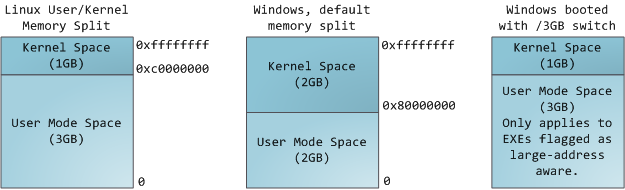
\includegraphics[width=1\columnwidth]{kernelUserMemorySplit}
	\captionsource{Répartition de l'espace mémoire du kernel}
	{Répartition de l'espace mémoire entre le noyau et le programme, par G.~Duarte}
	{\url{http://duartes.org/gustavo/blog/post/anatomy-of-a-program-in-memory/}}
	\label{fig:kernelUserMemorySplit}
\end{figure}

L'espace réserver au programme est ensuite découpé en différents segments tel que la Stack, Heap, etc. Ces segments sont des plages mémoires continues gérée par le système d'exploitation. Dans le cas d'un processus Linux les ségments sont répartit ainsi :

\begin{figure}[H]
	\centering
	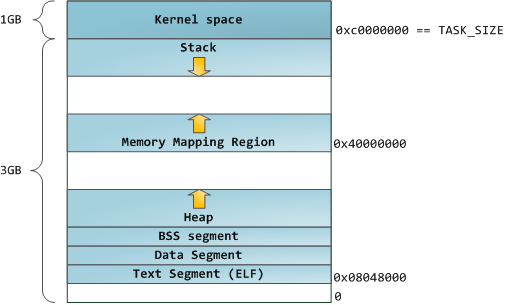
\includegraphics[width=.7\columnwidth]{linuxClassicAddressSpaceLayout}
	\captionsource{Ségmentation de la mémoire d'un processus Linux 32 bits}
	{Ségmentation de la mémoire d'un processus Linux 32 bits, par G.~Duarte}
	{\url{http://duartes.org/gustavo/blog/post/anatomy-of-a-program-in-memory/}}
	\label{fig:linuxClassicAddressSpaceLayout}
\end{figure}

La Stack permet de gérer le "Control-Flow" de l'application. À chaque appel de fonction, une nouvelle stack frame est ajoutée à la Stack et est ensuite retirée lorsque celle-ci se termine. La Stack grandit vers le bas, c-à-d que les adresses mémoires sont décroissantes. Il est possible que la Stack veuille s'étende au-delà de sa taille maximum, c'est le stack overflow et dans ce cas le programme recoit un "segmentation fault".

Le segment "Memory Mapping Region" permet au noyaux de copier en mémoire le contenu de certain fichier de manière à augmenter les performances. Ce segment est généralement utilisé pour charger les librairies. Il peut aussi être utilisé à d'autre fin, à la place de la Heap par exemple.

En dessous se trouve la Heap, permettant de stocker en mémoire les allocations dynamiques. En C ce ségment est géré par la fonction \mintinline{c}|malloc()| ainsi que ses collèges. Dans d'autres langages bénéficiant d'un ramasse mièttes tel que le C\#, l'interface pour intéragir avec la Heap est le mot reservé \mintinline{c}|new|.

Finalement les trois derniers segements que sont BSS, Data et Text servent a stocker les variables static initialisées ou non ainsi que la source du binaire executé. En \autoref{fig:mappingBinaryImage} un exemple de ce que l'on peut retrouver dans ces trois segments:

\begin{figure}[H]
	\centering
	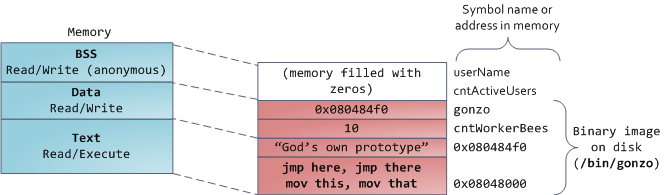
\includegraphics[width=.8\columnwidth]{mappingBinaryImage}
	\captionsource{Mapping d'une image binaire dans les ségments BSS, Data et Text}
	{Mapping d'une image binaire dans les ségments BSS, Data et Text, par G.~Duarte}
	{\url{http://duartes.org/gustavo/blog/post/anatomy-of-a-program-in-memory/}}
	\label{fig:mappingBinaryImage}
\end{figure}

Lors de l'execution d'un programme, cette mémoire virtuelle est gérée par le système d'exploitation grâce à une structure appelée "Memory Descriptor". Cette structure contient les adresses de début et de fin de chaque ségments.

\begin{figure}[H]
	\centering
	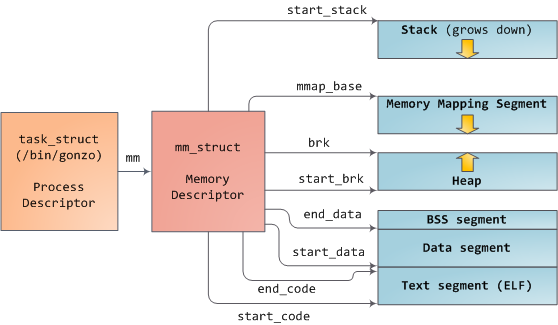
\includegraphics[width=0.6\columnwidth]{mm_struct}
	\captionsource{Memory Descriptor d'un processus Linux}
	{Memory Descriptor d'un processus Linux, par G.~Duarte}
	{\url{http://duartes.org/gustavo/blog/post/how-the-kernel-manages-your-memory/}}
	\label{fig:mm_struct}
\end{figure}

Cette structure est constituée d'une suite de \mintinline{c}{vm_area_struct}. Chacun d'eux est un espace continu en mémoire. Ils permettent de stocker des informations tels que les droits d'écriture et de lecture ou encore les droits d'execution. Ils stockent aussi si et quel fichier est copier en mémoire.

\begin{figure}[H]
	\centering
	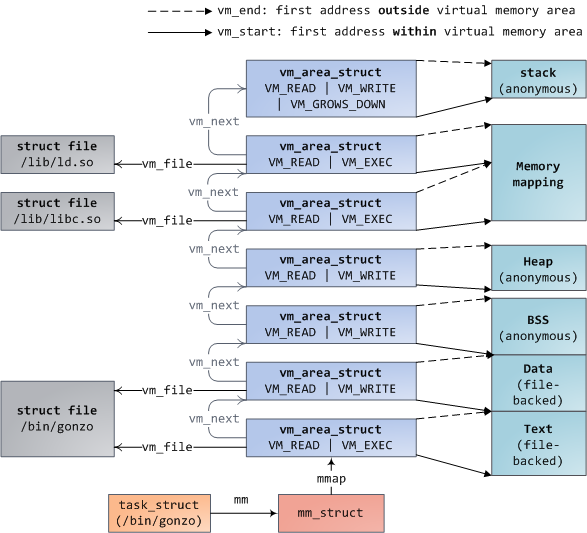
\includegraphics[width=1\columnwidth]{memoryDescriptorAndMemoryAreas}
	\captionsource{Structure des "Virtual Memory Area"}
	{Structure des "Virtual Memory Area", par G.~Duarte}
	{\url{http://duartes.org/gustavo/blog/post/how-the-kernel-manages-your-memory/}}
	\label{fig:memoryDescriptorAndMemoryAreas}
\end{figure}

% ---------------------------------------------------------------------------
\section{Le buffer overflow}

Le buffer overflow consiste à utiliser une fonction qui ne vérifie par la taille de l'argument à copier en mémoire, par exemple \mintinline{c}{strcpy()}, pour redéfinir l'adresse de retour de la fonction et modifier le flow de l'application en le redirigeant à un endroit ou l'attaquant aura, par exemple, péalablement injecter son code (p.ex. un shell code).

Lorsqu'une Stack frame est créée, celle-ci stocke dans un schéma particulier les informations d'ont elle a besoin.

\begin{enumerate}
	\item les paramètres passé à la fonction
	\item l'adresse de retour
	\item une sauvegarde du pointeur \%ebp
	\item et les variables locales
\end{enumerate}

Cela permet, en dépassant la taille des variables locales, de modifier des zones mémoires qui ne devraient pas l'être. En regardant la \autoref{fig:stackIntro} on constat que si l'on écrit (8+4+4+4) = 20 bytes dans le \mintinline{c}{local_buffer}, les 4 dernier bytes auront remplacé l'adresse de retour.

\begin{figure}[H]
	\centering
	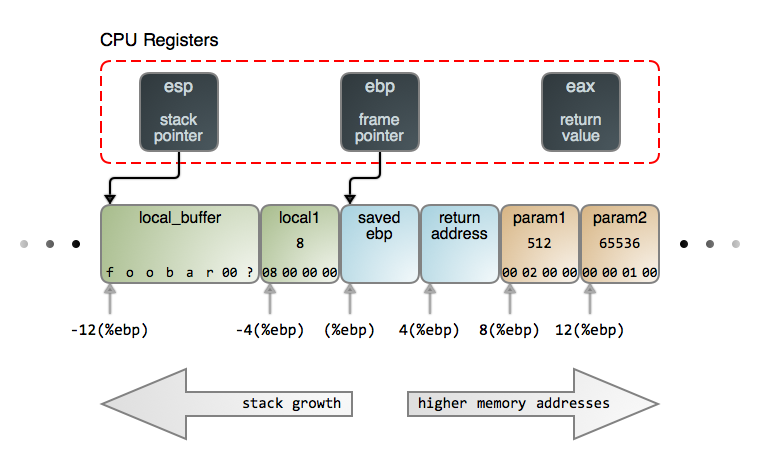
\includegraphics[width=1\columnwidth]{stackIntro}
	\captionsource{Exemple d'une Stack frame}
	{Exemple d'une Stack frame}
	{\url{http://duartes.org/gustavo/blog/post/journey-to-the-stack/}}
	\label{fig:stackIntro}
\end{figure}

Pour illustrer ce cas, voici un code C utilisant la fonction \mintinline{c}{strcpy()}. Dans cette exemple trivial il est possiblde d'injecter un shell code dans le buffer et de redefinir l'adresse de retour. La chaine de caractère copiée dans le \mintinline{c}{local_buffer} est directement contrôlée par l'utilisateur, ce qui rend la manoeuvre encore plus facile.

\usemintedstyle{monokai}
\begin{listing}
	\cfile{02-main/listings/buffer.c}
	\caption{Exemple de programe vulnérable au buffer overflow}
	\label{lst:buffer_overflow}
\end{listing}
\usemintedstyle{trac}


% ---------------------------------------------------------------------------
\section{DEP/NX}

Pour éviter lors d'un buffer overflow que l'attaquant puisse executer du code aux endroits mémoire censés contenir des données, les zones mémoires doivent être marquées comme étant executable ou non-executable. Cette information est justement stockée dans la structure "Virtual Memory Area" sour Linux.

\subsection{Mécanisme de protection}

DEP pour Data Execution Prevention a été introduit sur Linux en 2004 avec la version 2.6.8 du noyau, durant la même année pour Windows et deux ans plus tard pour Mac OS X lors de la transition vers x86 en 2006 \cite{DataExecutionPrevention}.

La protection se base sur le hardware, le NX bit, introduit tout d'abord par AMD en 2003, puis reprise par Intel sous le nom de XD bit une année après \cite{ExecutableSpaceProtection} \cite{NXBit}. Ce bit indique au processeur s'il sagit d'une zone d'instructions ou de données. Cependant cette fonctionalité hardware peut être simulée, entrainant du coup un overhead important.

\subsection{Contournements avec return-to-libc}

Une pile non-executable ne permet plus à l'attaquant d'executer son code, mais cela n'empêche pas d'executer du code executable déjà présent dans le programe. Comme montré dans la \autoref{fig:memoryDescriptorAndMemoryAreas}, la bibliothèque partagée libc est présente. Ce qui rend possible une attaque de type return-to-libc\cite{ReturntolibcAttack}. Grâce à la fonction \mintinline{c}{system()} il est possible d'executer arbitrairement un programe. Lors de l'attaque on localise par exemple une chaine de caractère tel que \mintinline{c}{"/bin/sh"} que l'on prepare comme étant le paramètre à passé à la fonction  \mintinline{c}{system()}.

% ---------------------------------------------------------------------------
\section{ASLR (Address space layout randomization)}

Comme montré sur la \autoref{fig:mappingBinaryImage}, l'espace d'adressage virtuel est structuré de manière fixe. De cette manière il est possible de prévoir ou se trouve en mémoir les différents composant de notre programe. L'attaque de type return-to-libc à besoin de connaitre l'adresse de la fonction \mintinline{c}{system()} et de la chaine de caractère \mintinline{c}{"/bin/sh"}. Dans le cas ou ces adresses changes à chaque lancement, la tâche devient plus compliquée.

\newpage

\subsection{Mécanisme de protection}

Depuis juin 2005, l'Address Space Layout Randomization est supportée dans le noyau Linux avec la version 2.6.12. Afin de rendre imprédictible les adresses sensibles, trois décalages aléatoires sont effectués au sein de la mémoire virtuelle. Le premier permet de décaler la Stack vers le bas, le second décale lui aussi vers le bas le segment de Mapping et le dernier décale vers le haut le segment de la Heap.

\begin{figure}[H]
	\centering
	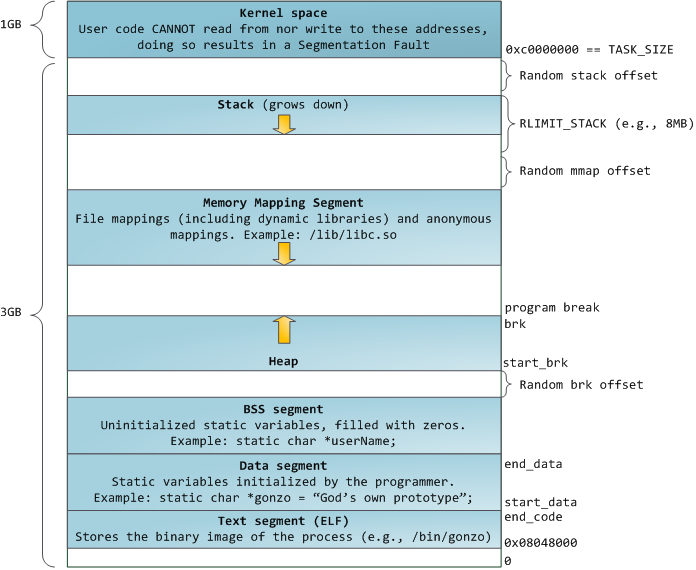
\includegraphics[width=1\columnwidth]{linuxFlexibleAddressSpaceLayout}
	\captionsource{Address space layout randomization}
	{Address space layout randomization}
	{\url{http://duartes.org/gustavo/blog/post/anatomy-of-a-program-in-memory/}}
	\label{fig:linuxFlexibleAddressSpaceLayout}
\end{figure}

\subsection{Limitation et contournements}

Sur un OS 32 bits, comme montré a la \autoref{fig:linuxFlexibleAddressSpaceLayout}, la marge de manoeuvre laissée au décalage n'est pas trés grande. Seul une partie des bits est utilisée, ce qui laisse possible une attaque de type force brutte réussir en quelques milliers d'essais. En effet la Stack est randomisée avec une entropie de 19 bits et la Memory Mapping 8 bits.

Dans le cas d'un OS 64 bits ASLR devient tout de suite plus interessant car l'espace mémoire virtuel est beaucoup plus grand. Cependant, les chercheurs Hector Marco-Gisbert et Ismael Ripoll de l'université de Valence ont écrit un papier démontrant une faiblesse sous certaines assomptions. \cite{EffectivenessFullASLR64bit}

% ---------------------------------------------------------------------------
\section{Les stack cannaries}




% ---------------------------------------------------------------------------
\section{Control-Flow integrity}



% \newpage

% % -------------------------------------------------------------------------
% This chapter shows example of picture and also serves to populate the different lists: list of figures, list of tables, bibliography, and glossary.
%
% \section{Tables}
%
% This section contains an examples of table: \autoref{tab:esempio}
%
% \begin{table}[H]
% 	\centering
% 	\begin{tabular}{ccc}
% 		\toprule
% 		name & weight & food \\
% 		\midrule
% 		mouse	& 10 g	& cheese \\
% 		cat	& 1 kg	& mice \\
% 		dog	& 10 kg	& cats \\
% 		t-rex	& 10 Mg	& dogs \\
% 		\bottomrule
% 	\end{tabular}
% 	\caption[A floating table]{A floating table.}
% 	\label{tab:esempio}
% \end{table}
%
% \section{Figures}
%
% This section contains examples of figures: \autoref{fig:galleria}, \autoref{fig:lorem}, \autoref{fig:ipsum}, \autoref{fig:dolor}, \autoref{fig:sit}
%
% \begin{figure}[H]
% 	\centering
% 	\includegraphics[width=0.5\columnwidth]{galleria_stampe}
% 	\captionsource{A floating figure}{A floating figure: the lithograph \emph{Galleria di stampe}, of M.~Escher}{\url{http://www.mcescher.com/}}
% 	\label{fig:galleria}
% \end{figure}
%
% \begin{figure}[H]
% 	\centering
% 	\begin{subfigure}[b]{0.45\textwidth}
% 		\includegraphics[width=\textwidth]{lorem}
% 		\caption{A gull}
% 		\label{fig:lorem}
% 	\end{subfigure}
% 	~ %add desired spacing between images, e. g. ~, \quad, \qquad, \hfill etc.
% 	%(or a blank line to force the subfigure onto a new line)
% 	\begin{subfigure}[b]{0.45\textwidth}
% 		\includegraphics[width=\textwidth]{ipsum}
% 		\caption{A tiger}
% 		\label{fig:ipsum}
% 	\end{subfigure}
% 	~ %add desired spacing between images, e. g. ~, \quad, \qquad, \hfill etc.
% 	%(or a blank line to force the subfigure onto a new line)
% 	\begin{subfigure}[b]{0.45\textwidth}
% 		\includegraphics[width=\textwidth]{dolor}
% 		\caption{A mouse}
% 		\label{fig:dolor}
% 	\end{subfigure}
% 	~ %add desired spacing between images, e. g. ~, \quad, \qquad, \hfill etc.
% 	%(or a blank line to force the subfigure onto a new line)
% 	\begin{subfigure}[b]{0.45\textwidth}
% 		\includegraphics[width=\textwidth]{sit}
% 		\caption{A mouse}
% 		\label{fig:sit}
% 	\end{subfigure}
% 	\caption{Example subcaption}\label{fig:animals}
% \end{figure}
%
%
% % -----------------------------------------------------------------------------
% \section{Code}
%
% \autoref{lst:listing_example} shows an example of Java code rendered with minted.
%
% \begin{listing}
% 	\javafile{02-main/listings/HelloWorld.java}
% 	\caption{Example of listing using the minted package}
% 	\label{lst:listing_example}
% \end{listing}
%
% % -----------------------------------------------------------------------------
% \section{Other features}
%
% Term (glossaries): \gls{nosql}
%
% Acronym (glossaries): \gls{sql}
%
% Citation (biblatex): \cite{paper_millwheel}
%
% % -----------------------------------------------------------------------------
% \section{Conclusion}
%
% \blindtext
